\subsection{Jetpack in general}
\label{cha:jetpack_general}

Jetpack is a set of many useful libraries which are used in Android development. It combines old and new libraries, therefore managing and updating gets much easier. As of 2018 when Jetpack got announced at the Google I/O one of the first steps was to rename the old \textit{android.support.*} libraries which are used for compatibility across multiple Android versions, to the new namespace \textit{androidx.*} \cite{allen2021introducingandroid}.

The components used in Jetpack are not bundled and each one must be imported explicitly. The available parts can be categorized into four categories, as shown in figure~\ref{fig:jetpack_components}. The categories are architecture, user interface, foundation and behavior. Which components are in which category is shown in the following figure:

\begin{figure}[ht]
  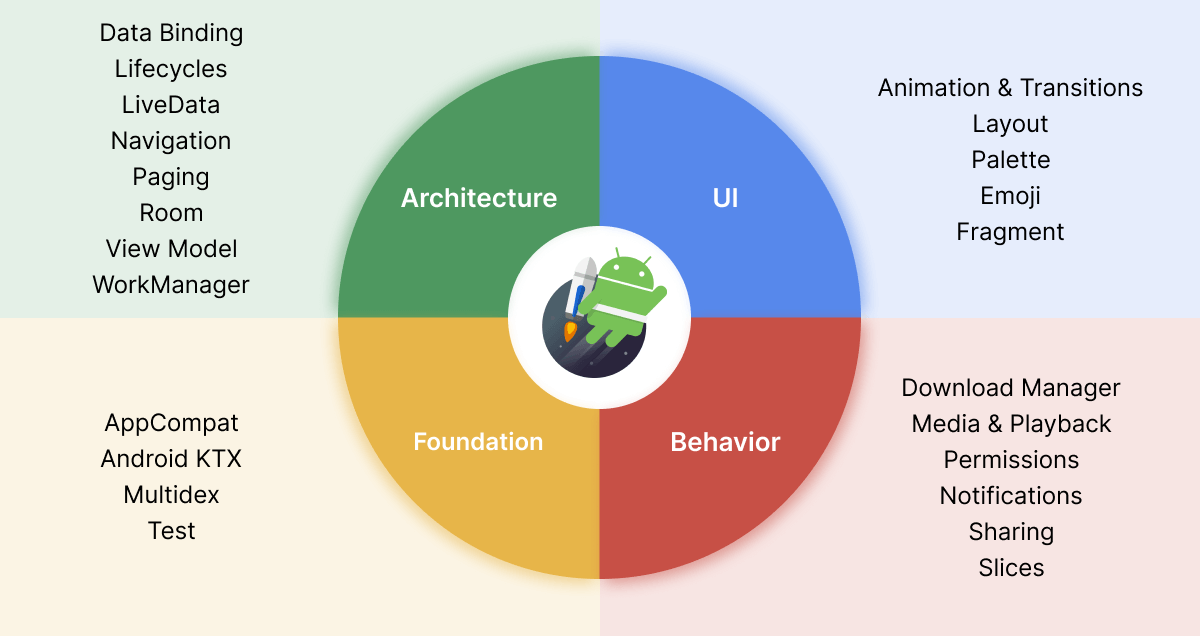
\includegraphics[width=\linewidth]{images/android-jetpack-components.png}
  \caption{Jetpack components and its categories \cite{Figure_1}}
  \label{fig:jetpack_components}
\end{figure}
% https://img.orangesoft.co/media/android-jetpack-components.png

One of the major goals of Jetpack is the integration with the programming language \textit{Kotlin}.
At the Google I/O 2019, Google announced the future development of Android will be written in Kotlin, because you can code more cleaner code than with the boilerplate language \textit{Java}. Kotlin and Java are 100\% interoperable, which means you can call Kotlin-code from Java and call Java-code from Kotlin \cite{android_kotlin_first}.
    
% \cite{android_jetpack_google}